\documentclass[12pt,a4paper]{report}
\usepackage[a4paper,hmargin={1in},vmargin={1in}]{geometry}
\usepackage{url}
\usepackage{graphicx}

% Code listing formatting. 
% Thanks to: https://www.sharelatex.com/learn/Code_listing
\usepackage{listings}
\usepackage{color}

\definecolor{codegreen}{rgb}{0,0.6,0}
\definecolor{codegray}{rgb}{0.5,0.5,0.5}
\definecolor{codepurple}{rgb}{0.58,0,0.82}
\definecolor{backcolour}{rgb}{0.95,0.95,0.92}

\lstdefinestyle{mystyle}{
	backgroundcolor=\color{backcolour},   
	commentstyle=\color{codegreen},
	keywordstyle=\color{magenta},
	numberstyle=\tiny\color{codegray},
	stringstyle=\color{codepurple},
	basicstyle=\scriptsize,
	breakatwhitespace=false,         
	breaklines=true,                 
	captionpos=t,                    
	keepspaces=true,                 
	numbers=left,                    
	numbersep=5pt,                  
	showspaces=false,                
	showstringspaces=false,
	showtabs=false,                  
	tabsize=2
}

\lstset{style=mystyle}
% End code listing formating.

% Title Page
\title{Internet Censorship Circumvention Network – Volunteer Relay Module}
\author{Edgar A. Cobos}
\date{Divide by Zero\\\today}



\begin{document}
\maketitle

\begin{abstract}
Freedom of speech and to information are essential for the development and further advancement of the human race. Freedom of speech gives the people power to readily speak up about injustices, corruption or express a dissenting point of views, without the fear of prosecution. On a similar note, freedom to information is what gives people the ability to read and view the broadcast of such injustices, corruption or dissenting point of views. Therefore, freedom of speech and to information provides a type of checks-and-balances between the people and governing body. In place to improve the quality of life. 


\end{abstract}

\renewcommand{\chaptername}{Section}
\tableofcontents

\chapter{Introduction}
The Internet’s ability to connect people and ideas gives it great power. Uniting minds from regions near and far. However, some people in power do not believe that sharing ideas is in their best interest. The fear lies in the result of what the masses will do in light of seeing governmental action that only favors those in power or a way of life that gives power to the people. As a result, there exists several countries with governing bodies that enforce Internet traffic filtering. Replacing search results that would otherwise reflect poorly on the country with those that make them look favorable, or all-together blocking website that show any dissent against the government. Since the government has control over the Internet service provides (ISP), they are able to implement packet filtering at the internet back bone level. This means that there is no way around the connecting gateway.In order to combat such censorship, we must go through the monitored gateway, undetected.

The Tor Project\footnote{\url{https://www.torproject.org/about/overview.html.en}} has developed the Tor Anonymous Network aimed at keeping users anonymous on the Internet. Most commonly, Chinese citizens use Tor to circumvent the infamous Great Firewall of China\footnote{\url{https://en.wikipedia.org/wiki/Great_Firewall}} The Tor Project has created a tool that is invaluable to those who wish to express themselves, but it is not without any flaws. The most notable flaw is the networks inability to properly support video streaming. The issue is caused by the network's structure. Interestingly enough, the same network structure that gives it its anonymous power is also what creates the noted flaw. So what does the inability to stream video content have to do with censorship? It means that users of Tor are limited to the kind of information they can access because Tor is only capable of supporting a subset of all available data. 
    
Tor works in the following way; a request is made, the data is relayed from an entry node to a middle node and lastly to an endpoint node, where the request is fulfilled. The network's issue lies with the amount of relaying needed to remain anonymous. Tor fully relies on other users volunteering are relays. Therefore, they are not able to enforce network requirement in order to become a relay for their network. Due to this fact, the time it takes to relay data from one node to the other is dependent on the underlying volunteers network. Its highly probably that volunteer are on subpar networks and will therefore add extra latency to the data delivery. We must also remember that there are at least three nodes that must be traversed, adding more latency, before the data packets reach their final destination. 

Our approach is to implement a network minimizes the number of relays the data has to traverse before reaching its final destination. Our goal is a bit different to that of the Tor Project's, we aim to solely circumvent censoring network by making users anonymous in the eyes of Internet service providers. Our network works in the following way: a request is made, a client application relays the data to a proper volunteer relay then lastly to a static proxy, which processes the request. As opposed to using three relays with potentially subpar internet speed, we use one. With speed in mind, the volunteer relay module application needs to run efficiently. Our goal is to keep the volunteers and network users satisfied with the performance. 


\chapter{Research}
The Tor anonymous network is the closest thing out there to this project. Just like this project, they rely heavily on people volunteering their machine as a relay for their network. They state on their website that the "more people that run relays, the faster the Tor network will be"[Tor Anonymous Network]. To an extent they are correct because the more people available to relay, the less time other have to wait for a connection or the more throughput bandwidth that is available. However, this still does not solve their issue of extended latency which prevents the proper streaming of video content. This is where our system will excel. Our network's end goal is to circumvent censoring intenet service provides by becoming anonymous to their monitors. This goal is different from Tor because they aim to make anyone anonymous on the internet. Since our goal is different, we are able to create a network that is able to go through filters undetected, while having low latency because of the smaller amount of relaying that is required. Our network will also run faster with the more people that volunteer but it is only because the available bandwidth throughput has increased. In either case, data will only need to go through one bottleneck, the volunteer relay, in order to get data packets from one end to the other. Tor on the other hand, requires at a minimum three volunteer nodes to complete its path. This means that data packets will hit up to three bottleneck throughout their journey from one end to the other.   

\chapter{Overview}
	
	\section{Problem Statement}
	As part of a circumvention network, the volunteer relay module is an application that will run on volunteering user's computer. The network heavily relies on the volunteer relays to complete a tunnel, for data transfer, from a client to an open internet endpoint. Open internet refers to the type of internet that provides unrestricted access to any available website. Therefore, it is absolutely crucial that the application be simple to use and install. Additionally, that it be disruption free to the volunteer or underlying host operating system. 
	 
	It should be the case that becoming a relay volunteer is simple and with minimal network setup. Once the relay service is turned on by the volunteer, it should become free of disruptions to the host system. This means that the application will need to run efficiently. On error, it will need to handle the error gracefully. We want to do everything we can to make volunteering favorable. The application should also be able to run on the Linux, Mac and Windows environments. 
	
	\section{Challenges}
	The first challenge was working with the Qt Creator Framework. It was my first time working with this framework, so there were a couple new concepts that I had to learn before being able to properly use it. Though it uses the C++ language for development, it requires that you abide by a specific syntax. Qt uses what they call Slots and Signals to handle function callbacks. I had to manually "connect" a signal to a slot on their respective object. A signal can be emitted by any function call, usually after some work of interest is complete. A slot is called when the signal is emitted and is then tasked with handling the callback. I ran into several issues with this concept initially because the paradigm was completely new to me. Since the Qt framework compiles an application for multiple platforms, I was forced to use wrapper data types and classes. Out of habit, I constantly used the non-wrapper data types and classes, which led to issues.      
	
	The application is both a server and client. For the privacy of a users we want to create encrypted links between a client to our application and from our application to the static proxy. This meant that I had to use SSL sockets with the corresponding OpenSSL library. My original goal was to use the latest OpenSSL library, version 1.0.2e. However, Qt did not make integrating the library easy.
	
	As a client, the application had troubles connecting to the static proxy via an SSL socket because it was not able to verify the proxy's certificate. The static proxy does have a certificate but it is self-signed by myself. This is fine while it undergoing further development. However, the issue is that Qt would refuse to make a connection because it was not able to verify its validity with a Certificate Authority. 
	
	Since the application is going to be handling several connection at once, it would make sense to fork on each new incoming socket connection. The reason for this is that each connection should be independent of the others. If one socket is using up more resources than it should, then it should have no impact on the other connections. Unfortunately, based on Qt's documentation, fork() is not available because Windows does not support such operation. 
	
	\section{Solutions}
	I used the Qt Creator Framework version 5.5 to develop the volunteer relay application. Qt has been around for over 20 years and it seems to be the go-to framework for cross-platform development. Qt has been around for so long that I felt confident starting a project on their framework and not have to worry about future support. Additionally, Qt is documented\footnote{\url{http://doc.qt.io/qt-5/gettingstarted.html}} extensively and even provides several examples\footnote{\url{http://doc.qt.io/qt-5/qtexamplesandtutorials.html}} that can be downloaded. The documentation was especially helpful initially when I was trying to figure out how things worked.
	
	Originally, I my goal was to use the latest version of OpenSSL because it provides support for the TLSv1.2 protocol. Qt made it really difficult to incorporate the desired library. Their instructions for including the library involved complex steps to compile the program. It was more involved than time allowed. Therefore, I decided to just stick with the OpenSSL library that comes out of the box with Qt, version 0.9.8. Unfortunately, that version only support the TLS protocol up to version 1.0. However, this protocol is good for now, while the prototype is being developed. 
	
	We ended up purchasing a certificate, signed by a valid Certificate Authority. However, before purchasing the certificate, I had to do something called certificate pinning, on the the application. Essentially, I took the static proxy's self-signed certificate and imported it into the volunteer application. Programmatically, I had to tell Qt that it should trust the certificate that I added into its resources. Once that was complete, Qt had no troubles connecting the static proxy. 
	
	As it turns out, Qt does not support the use of fork() because Windows does not have fork. In this case, my other option is to use threads. Threads are not the idea solution for our issue since they are all still running under the same process. An issue in one thread may affect the others. In addition to threads, the application makes use of slots and signals to handle connections. Whenever new data is written into the incoming socket buffer, a signal is emitted then a slot reads the buffer data and immediately writes it to the destination socket buffer. The slots and signals ensures that data is being moved from one socket buffer to another to prevent a backup or worse, overwriting.   
	
	\section{Individual Work}
	My work includes everything related to the volunteer relay module. Once a user starts the volunteer relay, the application will connect to an external server to fetch the information needed to make a connection to the static proxy. That information is retrieved as JSON data then parsed for later use. The Qt Framework provides a QTcpServer class, which I had to extend to implement an SSLServer class. The goal of extending the class was to accept incoming SSL connections with my specified parameters. Here I was able to specify that the server will only accept TLSv1 protocol connections. Since we have control over the client module, I was able to enforce that restriction with confidence. Once an SSL connection is accepted, the application then has to make another TLSv1 connection to the static proxy. By this time, we should already have the static proxy's IP and port. On success, a tunnel from the client module to the static proxy is established. The tunnel is marked successful once the client module completes a key exchange handshake with the static proxy. 
	
	I initially created three main classes; one controller, a client connection class and a static proxy connection class. The client connection class was essentially the SSL server that accepted incoming connections from clients. The static proxy connection class would act as the client to connect to the static proxy server. Lastly, the controller class would handle reading data from a client socket then write it to a proxy socket, and vice-versa. Later, I figured that this structure would involve several constant, yet unnecessary, method calls to both the client and proxy objects. With that in mind, I had to give up the notion of low coupling in preference of speed. I had to structure the classes in a way where there would be minimal function calls. In the end, the client class now directly creates a static proxy object that it can use with slots and signals to handle the socket buffer data events. Essentially, I cut out the middle man, the controller class.       
	
	\section{Comparing my work with teammates}
	I worked on this project alone so I do not have any one I can compare against. There are always things I can improve upon but some that need more focus are time management, fully reading the documentation and brush-up on my C++ skills. Time seemed to always be an issue for me. I was constantly focused on trying to meet hard deadlines for other classes to a point where this project would get little attention. I did allocate equal amounts of time for all my projects but I had a hard time sticking by those time allocation. One project would not work as expected and as a result it would require more time which was taken away from this project's progress. Also because of the time constraint, I never fully read the Qt documentation, only what was required to get the program to work. It is likely not a big issue but I would still like to improve in that respect. There were times that I would spend a lot of time trying to figure something out only to find out that the answer I sought was on the same previously visited documentation page. Lastly, C++ is rarely ever used outside of the C++ course and because of that I struggled initially with trying to remember how C++ operates. It is not to say that I was not capable of writing proper C++ code, it is more along the lines of getting situated with the language. Java, which is heavily used, does not explicitly use the concept of header files and implementation files. I had to pull out my old C++ book to brush up on pointers, memory management and data type sizes. As someone that is about to graduate with a computer science degree, I should know C++ like the back of my hand.     
	
	
	\section{Shortcomings}
	I did not get everything that I wanted done because I had to spend some time working on the other modules that interact with this application. The application is one piece to the bigger network, but it has to be able to properly interact with the other modules. When the application ran as a client, I ran into a couple issues with the static proxy module. I had to update the static proxy's code so that it would properly accept connections from this new intermediary source. The cause of this issue is that the static proxy was created so that it connect to the client directly. It was decided at the time, that a direct connection was fine just to get the project moving along. It was assumed that integrating the volunteer relays would have been simple.To an extent, the integration was mostly easy. When the application ran as a server, the client module was not able to connect because an HTTPS connection was expected. The client module was not created with the ability to make HTTPS connections and thus the TLSv1 handshake would fail. I had to spend some time working on the client module so that it would be able to connect via an SSL socket.
	
	 
	\section{Lessons Learned}
	Through this project I learned several concepts that are not taught within the CSULB computer science curriculum. I learned that the Qt framework is a pain to work with initially, but once the concepts of Qt are understood, the power of it shines through. The frameworks limitations force to learn about the certificate pinning concept. I am truly grateful that their documentation is of high quality. It showed me the value of well documented code. Because of the documentation, I was able to figure out that if I wanted to become a secure server, I had to extend X, Y and Z. This is in contrast to other languages where such an obstacle requires extensive Google search. This was also my first time creating a GUI application that natively ran on my computer. After some research, I found out that those are common concepts with GUI related applications. So now I can say that I understand how slots and signals work, or triggers and callbacks, as they are called elsewhere.
	
	Overall, I really enjoyed the course project. I do feel that projects push me to learn new things. The best part about learning new things is that one does not realize the amount of learning that is going on until its time to reflect on what was accomplished. The thing that I disliked about the project was the amount of time it took to get simple things to work properly. Though I did learn along the way, I found it frustrating to get past one hurdle only to be face with another one. I understand that such is a programmers life, I just do not have much to dislike about the course project. I like to learn and I like to make cool things.  

	
\chapter{Implementation}
 The implementation code for this project is located in the Appendix section. Since I worked on this project alone, I did not want to place the same code in two different locations, unnecessarily taking up space. Just to reiterate, I worked on the volunteer relay module for this project. As you can see from Figure 4.1, the module lies between a client module and a proxy.  
 
\begin{figure}[h]
 	\caption{Overview of the full system}
	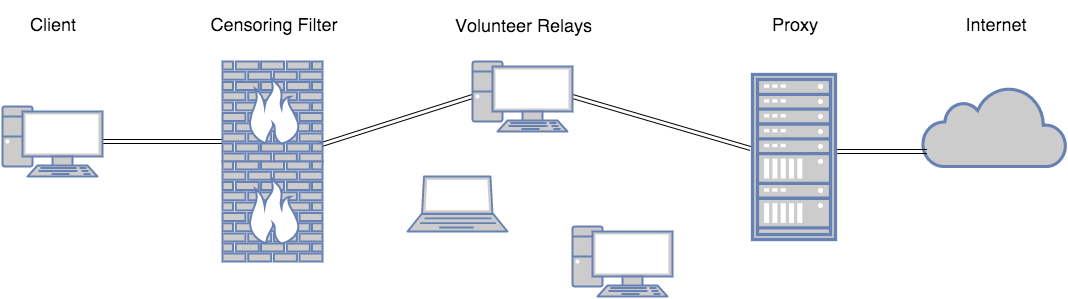
\includegraphics[width=\textwidth]{BigPicture.png}
\end{figure}

There are several interactions that happen behind the scenes for network. Figure 4.2 shows at a high level all the steps that must be taken before a secure tunnel from a client module to the proxy, can be made. 
\begin{figure}[h]
	\caption{Volunteer Relay Flowchart}
	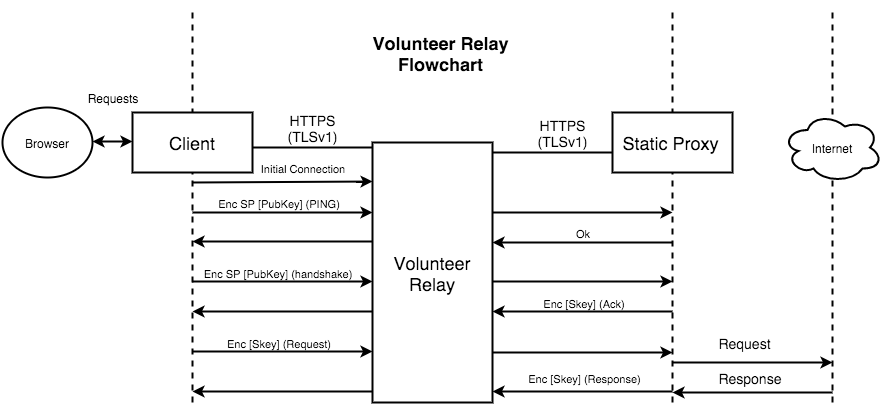
\includegraphics[width=13cm, height=5cm]{VolunteerRelay.png}
\end{figure}
I did not have much time to get everything that I wanted working, but I did get the handshake between the client and the static proxy to work properly. This is the first step with getting the volunteer relay module working properly. These results indicate that my initial code is working well enough for prototyping purposes. 
\begin{figure}[h]
	\caption{Connecting from the Client Module}
	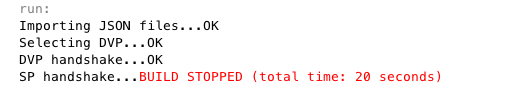
\includegraphics[width=9cm, height=2cm]{client.png}
\end{figure}
\begin{figure}[h]
	\caption{Operations occuring in the volunteer relay module}
	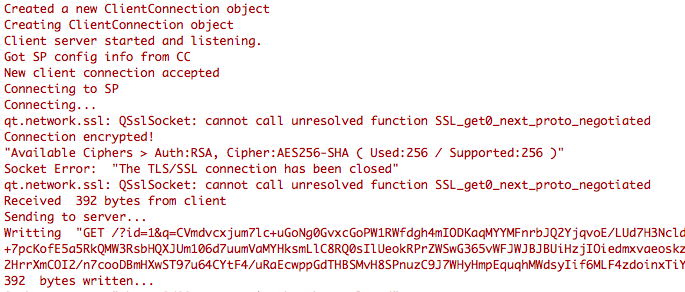
\includegraphics[width=10cm, height=4cm]{dvp.png}
\end{figure}
 
 \begin{figure}[h]
 	\caption{Connection on the static proxy module}
 	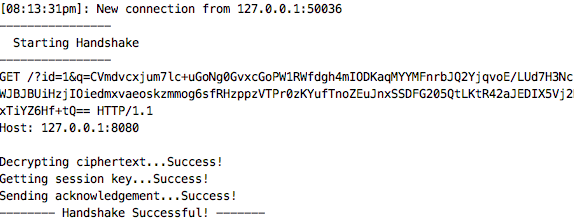
\includegraphics[width=10cm, height=4cm]{SP.png}
 \end{figure}
 
\chapter{Conclusion and Future Work}
There are a couple things that I did not have time to implement but are essential to the module. The  first is to stabilize the connection between the client module and the static proxy. I was having some troubles with dependencies on my working computer, so I did not get the time to fully test the robustness of the application. I also would like to test the application with multiple incoming connections. So far, my test have only included one connection from me, but I would like to see how well it can handle maybe 10 simultaneous connections. Since we want the application to be volunteer friendly, I want to add more features to the GUI. Showing the user how much data is being relayed through their application would allow them to decide if they want to volunteer less. The user knows his or her connection speeds, so they are more capable to decide the amount of resources they are willing to offer at any given point. This also means that the GUI will need to support some throttling functionality. The application is likely going to site behind personal firewalls, so I will need to do some research on how to make this easy for the user. Lastly, the application will be distributed and used by anyone who wishes to volunteer their bandwidth. With that in mind, we need to assume that the volunteer is untrusted because we do not know their intentions or ability to modify our application in an unintended manner. I will need to do some further research but having something that disallows the tampering of the application code would be ideal. Even using some kind of trap that renders the application useless if its tampered. 
\chapter{Bibliography/Citation}

Hani. "How a Client App Connect to an SSL Server with a Self-signed Certificate in Qt?" Ed. Marco.m. Stack Overflow, 15 Sept. 2013. Web. 11 Dec. 2015. [http://stackoverflow.com
/questions/18810788/how-a-client-
app-connect-to-an-ssl-server-with-a-self-signed-certificate-in-qt].
\\\\
"Signals and Slots | Qt Core 5.5." Qt Framework, n.d. Web. 11 Dec. 2015. 
[http://doc.qt.io/qt-5.5/signalsandslots.html];.
\\\\
"QSslSocket Class | Qt Network 5.5." Qt Framework, n.d. Web. 11 Dec. 2015. [http://doc.qt.io/qt-5/qsslsocket.html].
\\\\
"Tor Anonymous Network." Tor Project, n.d. Web. 11 Dec. 2015.
[https://www.
torproject.org/about/overview].


\chapter{Appendix} 
 \lstinputlisting[language=C++, caption=Controller.cpp]{./Controller.cpp}
 \lstinputlisting[language=C++, caption=ClientConnection.cpp]{./ClientConnection.cpp}
 \lstinputlisting[language=C++, caption=StaticProxyConnection.cpp]{./StaticProxyConnection.cpp}
\end{document}          
